Simulations results using $K_\omega=500$:

% d0 Controller
\begin{figure}[H]
    \centering
    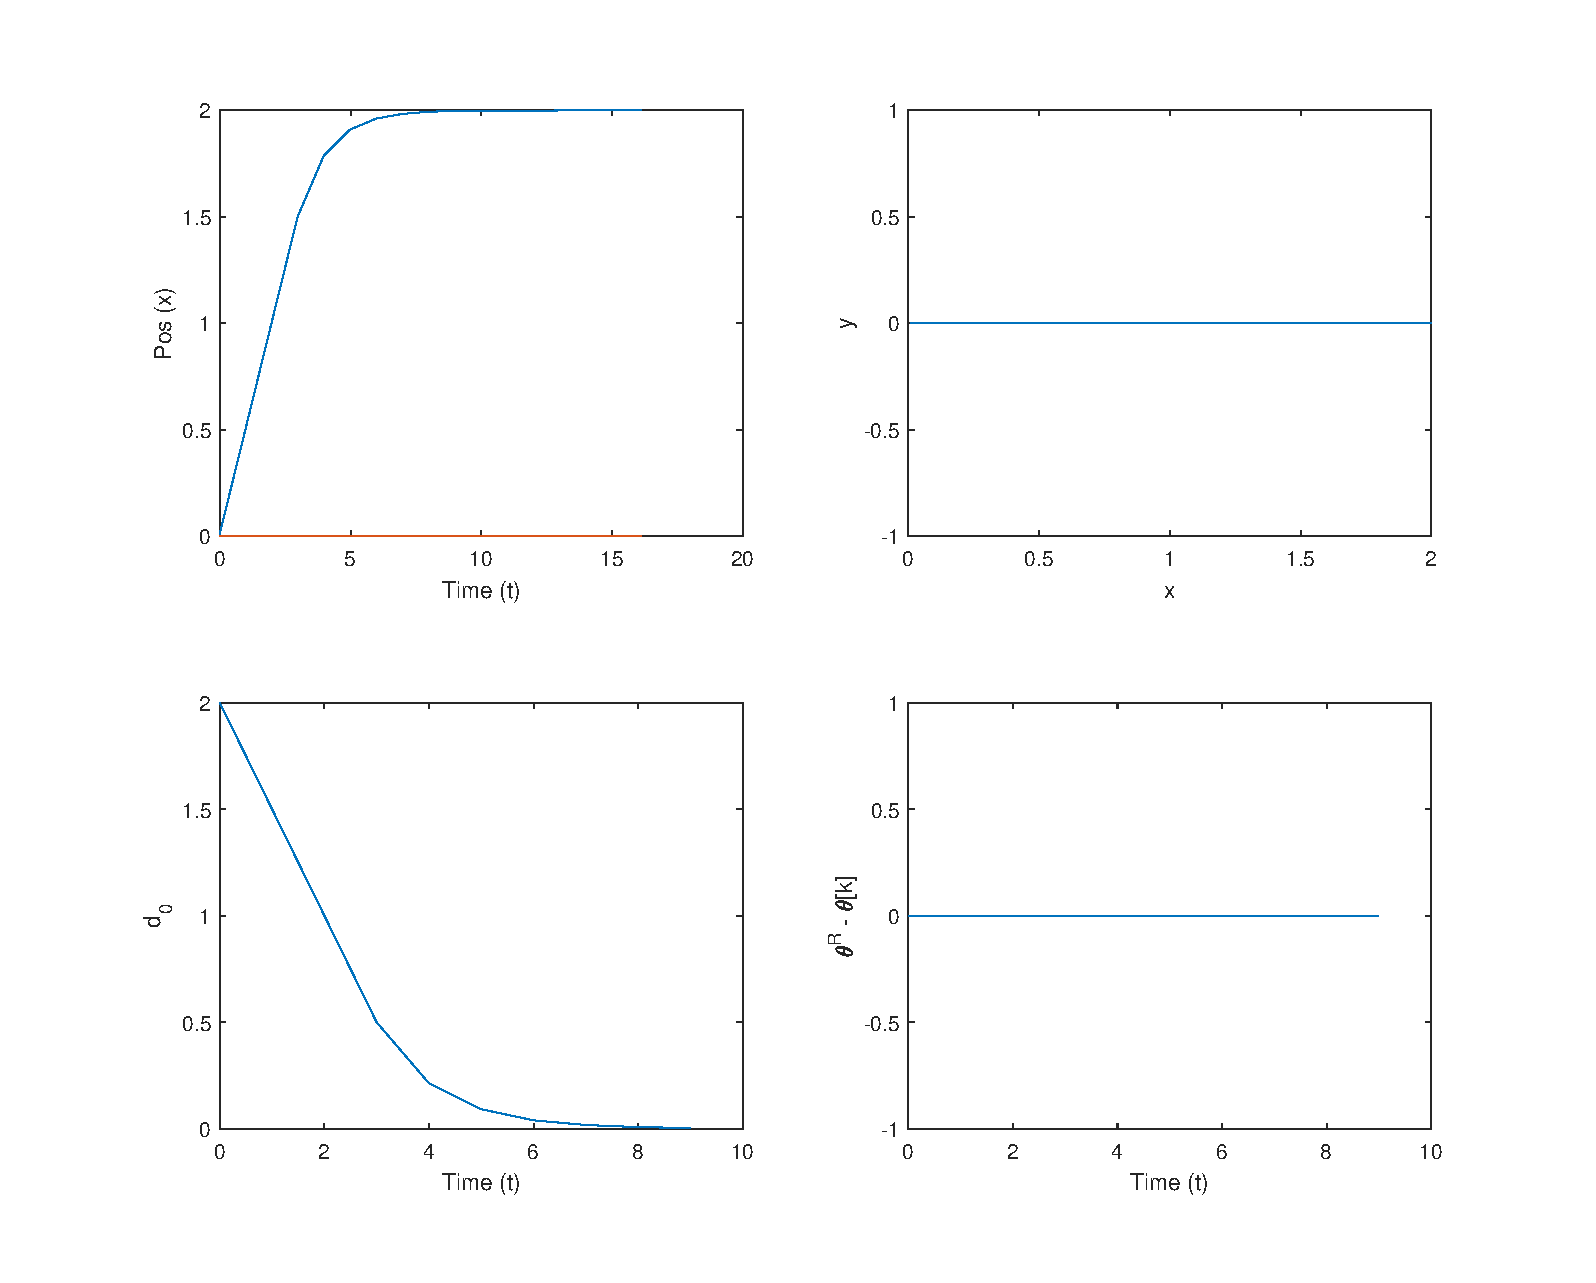
\includegraphics[width=\textwidth]{figs/perf-d0.eps}
    %\begin{subfigure}[b]{7cm}
    %    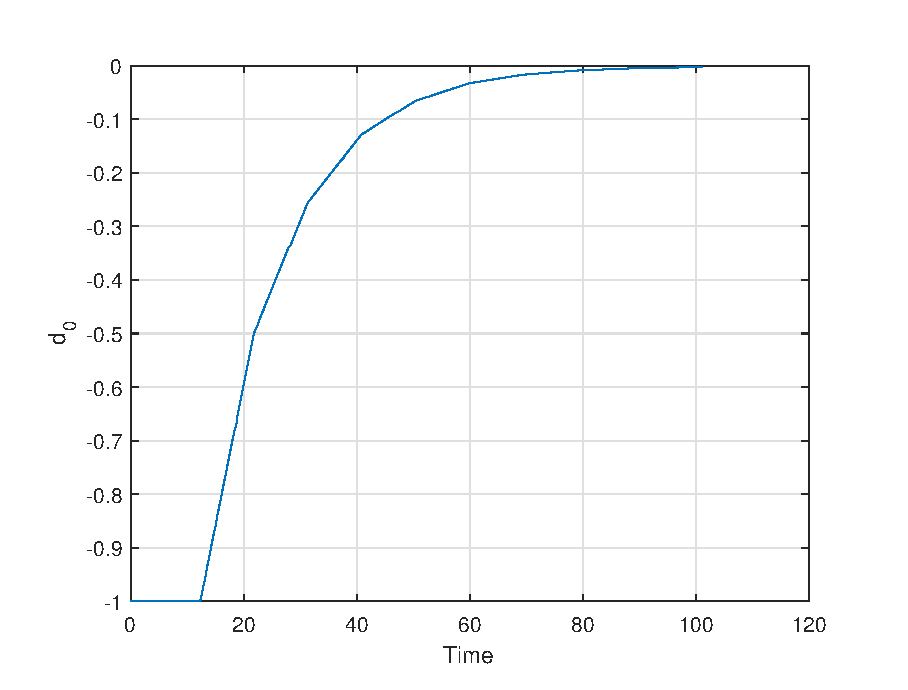
\includegraphics[width=\textwidth]{task8_500_d0_initial_00_Goal_11.eps}
    %    \caption{Initial position: (0,0), Goal: (1,1)}
    %    \label{fig:500d00011}
    %\end{subfigure}
    %\begin{subfigure}[b]{7cm}
    %    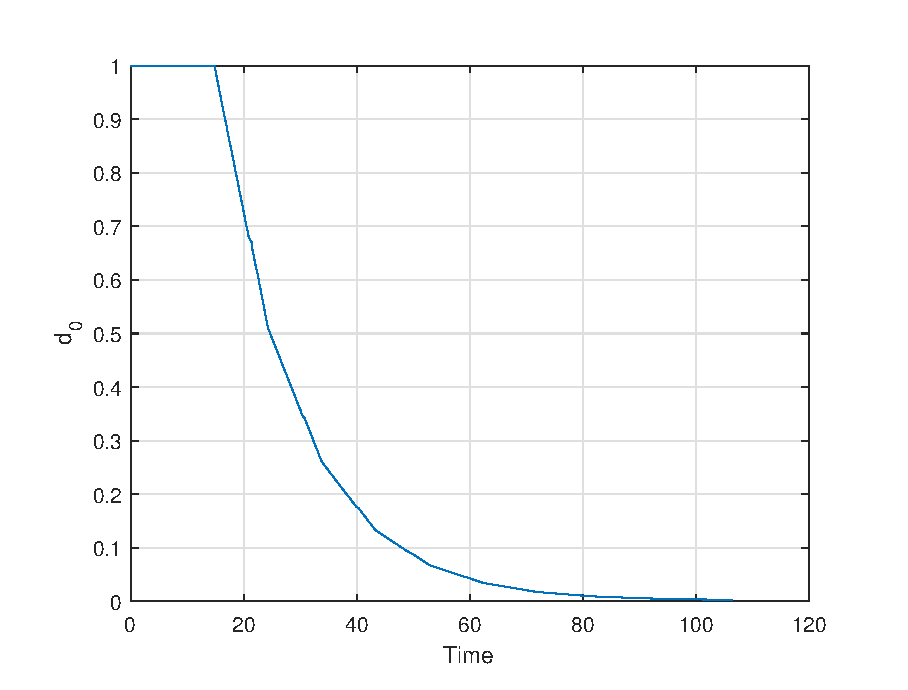
\includegraphics[width=\textwidth]{task8_500_d0_initial_21_Goal_11.eps}
    %    \caption{Initial position: (2,1), Goal: (1,1) }
    %    \label{fig:d05002111}
    %\end{subfigure}
    %
    %
    %\begin{subfigure}[b]{7cm}
    %    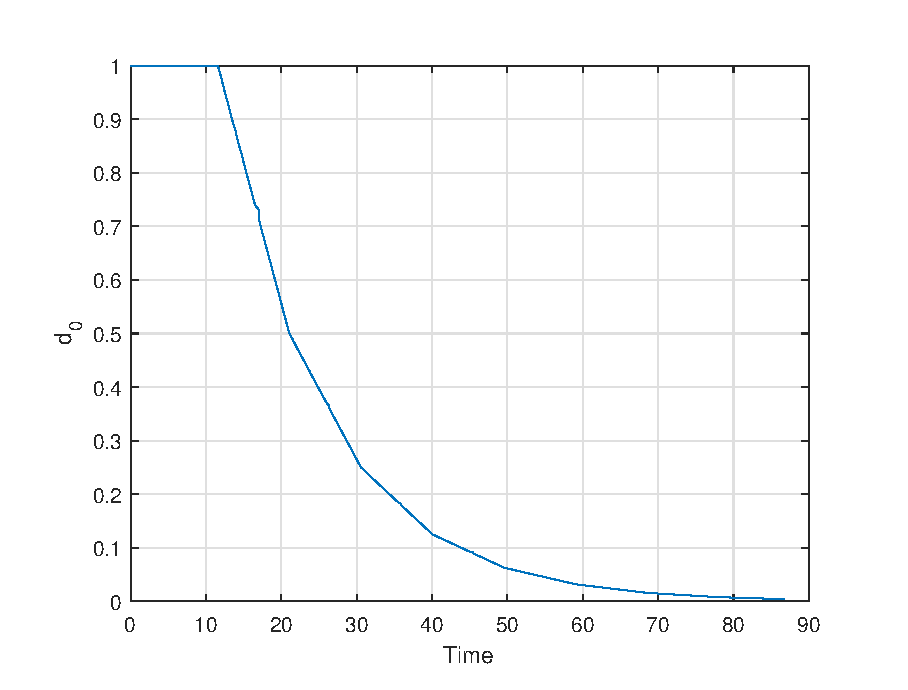
\includegraphics[width=\textwidth]{task8_500_d0_initial_11_Goal_02.eps}
    %    \caption{Initial position: (1,1), Goal: (0,2)}
    %    \label{fig:d05001102}
    %\end{subfigure}
    % \begin{subfigure}[b]{7cm}
    %    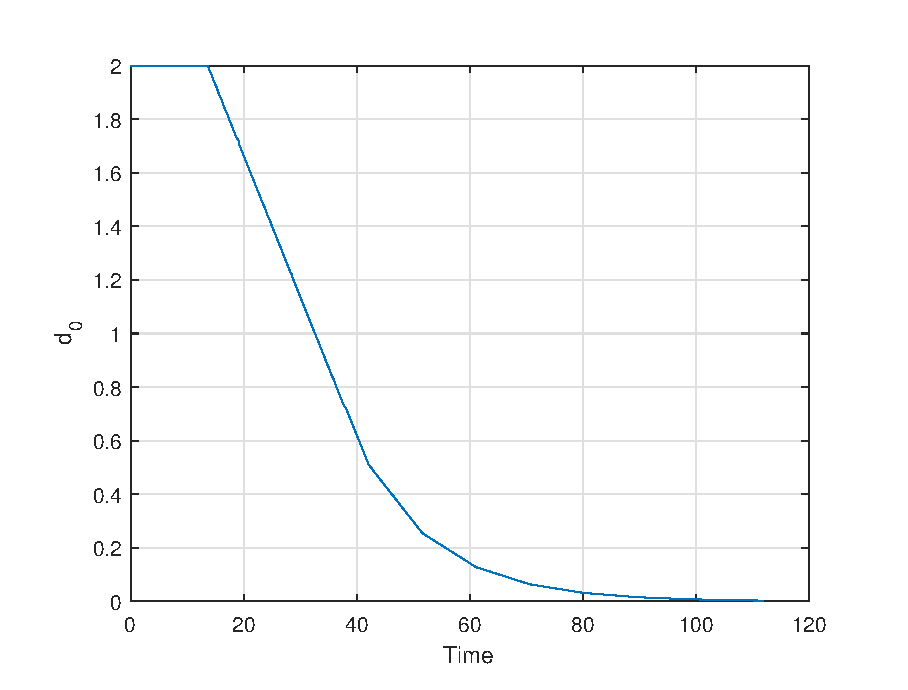
\includegraphics[width=\textwidth]{task8_500_d0_initial_20_Goal_02.eps}
    %    \caption{Initial position: (2,0), Goal: (0,2) }
    %    \label{fig:d05002002}
    %\end{subfigure}
    
    \caption{Simulation of the $d_0$ controller going from $(0, 0)$ to $(2, 2)$ with $K_\omega= \frac{180}{R \pi}.$}\label{fig:d02002}
\end{figure}

The controller drives the robot to a position orthogonal to the goal position where the value $d_0$ is zero. If the robot is aligned with the line from the initial position to the goal, then the robot will reach the goal position. Otherwise it will not.\textbf{}